\documentclass[a4paper,10pt]{book}
\usepackage[utf8]{inputenc}
\usepackage{graphicx}
\usepackage{amsmath}
\usepackage{esint}

%opening
\title{}
\author{}

\begin{document}
\chapter{22 de agosto}

\section{Encontros}

* Preferem horários fixos. 
* Enquete no moodle sobre horários.

\section{Questões}
\begin{eqnarray*}
 \vec{u} &=& u_1\vec{i} + u_2\vec{j} + u_3\vec{k}\\
 \vec{v} &=& v_1\vec{i} + v_2\vec{j} + v_3\vec{k}
\end{eqnarray*}

Como $\vec{u}$ e $\vec{v}$ estão no plano XY, $u_3=v_3=0$. 

Como $\|\vec{v}\|=0$, $\vec{v}=\vec{0}$.

Já $\vec{u}$ é unitario, então $u_1^2+u_2^2=1$.
$$u_1=\cos(\theta),~~u_2=\sin(\theta).$$

Obs.: Quando $\theta=0$, $\vec{u}=\vec{i}$.
Quando $\theta=\pi/2$, $\vec{u}=\vec{j}$,

\section{Produto misto}
\begin{eqnarray*}
 \vec{u}\times  \vec{v} \cdot \vec{w}=(\vec{u}\times  \vec{v}) \cdot \vec{w}=\underbrace{\vec{u}\times(  \vec{v} \cdot \vec{w})}_{ERRADO}
\end{eqnarray*}


\begin{eqnarray*}
\vec{u}&=&\vec{i}+2\vec{j}+3\vec{k}\\
\vec{v}&=&\vec{i}       -\vec{k}\\
\vec{w}&=&\vec{i}+2\vec{j}+\vec{k}\\
\end{eqnarray*}

\begin{eqnarray*}
\left|\begin{array}{ccc}
1&2&3\\       
1&0&-1\\
1&2&1
      \end{array}
\right| = 1\cdot 0 \cdot 1 + 2\cdot(-1)\cdot1 + 3\cdot 1\cdot 2 - 3\cdot 0\cdot 1 - 2\cdot 1\cdot 1 - 1 \cdot (-1) \cdot 2
\end{eqnarray*}

\section{Ângulo entre vetores}

Usaremos:
$$\vec{u}\cdot\vec{v} = \|u\|\|v\|\cos(\alpha)$$
$$|\vec{u}\times\vec{v}| = \|u\|\|v\|\sin(\alpha)$$


\section{Funções vetoriais}

$$\vec{u}(t) = u_1(t)\vec{i}+u_2(t)\vec{j}+u_3(t)\vec{k}$$

Exemplo: vetor posição.
$$\vec{r}(t) = x(t)\vec{i}+y(t)\vec{j}+z(t)\vec{k}$$

A velocidade é a derivada:
$$\vec{v}(t) = x'(t)\vec{i}+y'(t)\vec{j}+z'(t)\vec{k}$$

Teorema:
Se $\|\vec{r}(t)\|$ é constante, então:
$$\vec{r}(t)\cdot \vec{r}\!~'(t)=0$$


Aplicação na cinemática:
Se a velocidade de uma partícula tem módulo constante, isto é, velocidade escalar constante, então:
$$\vec{v}(t)\cdot \vec{v}\!~'(t)=\vec{v}(t)\cdot \vec{a}(t)=0$$

Generalização:
Se $\vec{v}(t)=v(t)\vec{T}(t)$
onde $\vec{T}(t)$ é o vetor tangente unitário dado por:
$$\vec{T}(t) = \frac{\vec{r}~\!'(t)}{\|\vec{r}~\!'(t)\|} $$

Diferenciando, temos:
\begin{eqnarray*}
 \vec{a}&=&\vec{v}~\!'(t)=\frac{d}{dt}\left[v(t)\vec{T}(t)\right]\\
 &=&\underbrace{v'(t)\vec{T}(t)}_{tangencial}+\underbrace{v(t)\vec{T}'(t)}_{normal}
\end{eqnarray*}
Observação. Como $\|\vec{T}(t)\|=1$, o teorema citado anteriormente garante que $\vec{T}(t)\cdot\vec{T}'(t)=0$.

\section{Curvatura}
A curvatura de uma curva descrita por $\vec{r}(t)$ é dada por:
$$\kappa(t) = \left\|\frac{d}{ds}\vec{T}(s)\right\|$$
onde $s(t)$ é o comprimento da curva.

\subsection{Circunferência}

\begin{eqnarray*}
\vec{r}(t)&=&\cos(t)\vec{i}+\sin(t)\vec{j} \\
\vec{r}~\!'(t)&=&-\sin(t)\vec{i}+\cos(t)\vec{j} \\
\|\vec{r}~\!'(t)\|&=&\sqrt{\sin^2(t)+\cos^2(t)}=1 \\
\end{eqnarray*}
Assim:
$$\vec{T}(t) = \frac{\vec{r}~\!'(t)}{\|\vec{r}~\!'(t)\|}=-\sin(t)\vec{i}+\cos(t)\vec{j}.$$
\begin{eqnarray*}
\kappa(t) &=& \left\|\frac{d}{ds}\vec{T}(s)\right\|\\
&=&\left\|\frac{d}{dt}\vec{T}(t)\right\|/ \frac{ds}{dt}\\
&=&\left\|\frac{d}{dt}\vec{T}(t)\right\|/ \|\vec{r}~\!'(t)\|\\
&=&\left\|\frac{d}{dt}\vec{T}(t)\right\|\\
&=&\left\|-\cos(t)\vec{i}-\sin(t)\vec{j}\right\|=1\\
\end{eqnarray*}


\chapter{24 de agosto}
\section{Vetores $\vec{T}$-$\vec{N}$-$\vec{B}$ (24/agosto)}
\begin{center}
 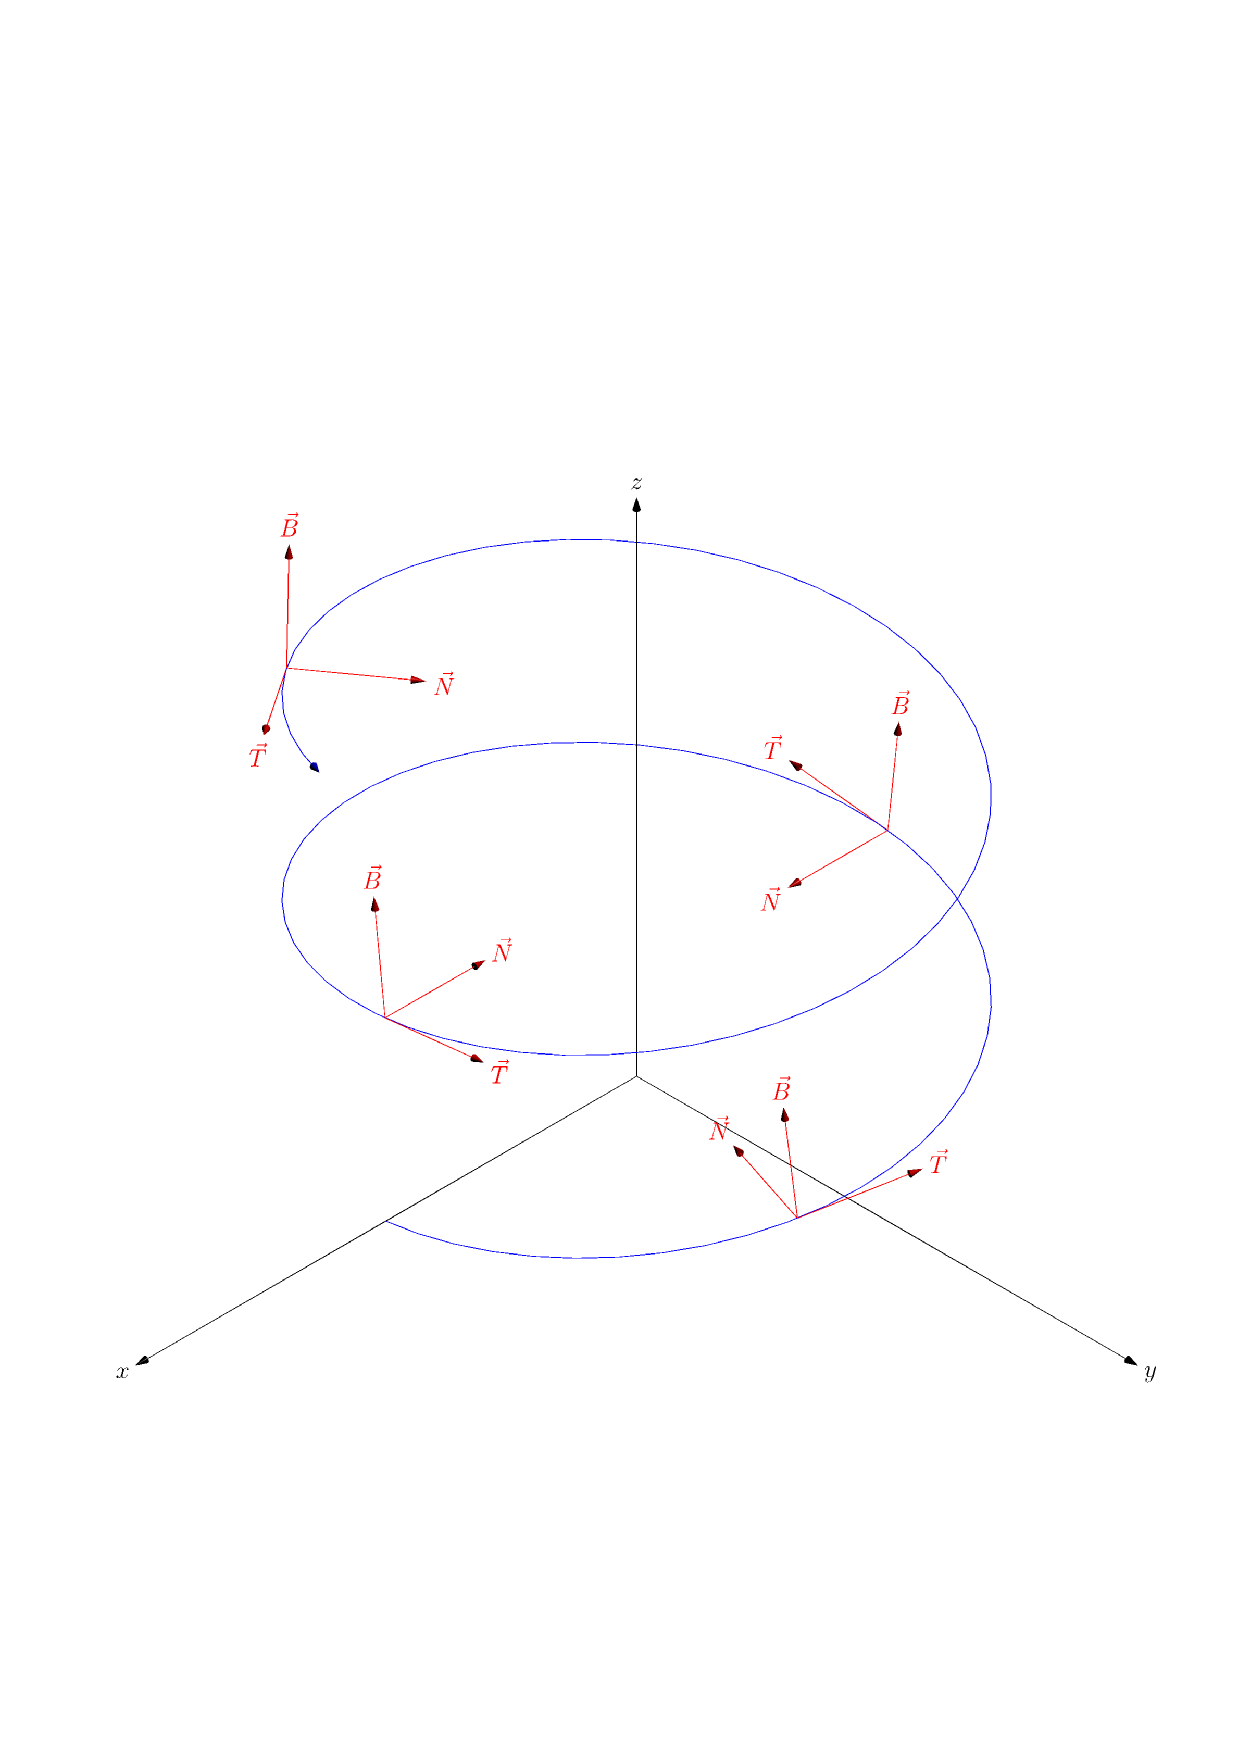
\includegraphics[width=7cm]{figs/helice_TNB.png}
 \end{center}

 \subsection{Vetor tangente unitário}
 Se uma curva é parametrizada pela função $\vec{r}(t)=x(t)\vec{i}+y(t)\vec{j}+z(t)\vec{k}$.
 
 Definimos o vetor tangente unitário:
 $$\vec{T}(t) = \frac{\vec{r}~\!'(t)}{\|\vec{r}~\!'(t)\|},~~\vec{r}~\!'(t)\neq \vec{0}.$$

 
 \subsection{Vetor normal unitário}
 Definimos o vetor normal unitário como:
 $$\vec{N}(t) = \frac{\vec{T}~\!'(t)}{\|\vec{T}~\!'(t)\|},~~\vec{T}~\!'(t)\neq \vec{0}.$$

  Obs: $\vec{N}(t)\cdot \vec{T}(t)=0$ porque $\vec{T}(t)$ tem norma constante. 
 

 
\subsubsection{Aplicação na cinemática}
Se a velocidade de uma partícula é a função $\vec{v}(t)$, então podemos escrever:
 $$\vec{v}(t)=v(t)\vec{T}(t)$$
onde $\vec{T}(t)$ é o vetor tangente unitário dado por:
$$\vec{T}(t) = \frac{\vec{r}~\!'(t)}{\|\vec{r}~\!'(t)\|}=\frac{\vec{v}(t)}{\|\vec{v}(t)\|} $$

Diferenciando, temos:
\begin{eqnarray*}
 \vec{a}&=&\vec{v}~\!'(t)=\frac{d}{dt}\left[v(t)\vec{T}(t)\right]\\
 &=&\underbrace{v'(t)\vec{T}(t)}_{tangencial}+\underbrace{v(t)\vec{T}'(t)}_{normal}
\end{eqnarray*}
Como $\vec{N}(t) = \frac{\vec{T}~\!'(t)}{\|\vec{T}~\!'(t)\|}$, obtemos:
\begin{eqnarray*}
 \vec{a}&=&\underbrace{v'(t)\vec{T}(t)}_{tangencial}+\underbrace{v(t)\|\vec{T}~\!'(t)\|\vec{N}(t)}_{normal}
\end{eqnarray*}
 
\subsection{Vetor binormal unitário}
O vetor binormal unitário é definido como:

 $$\vec{B}(t)=\vec{T}(t)\times\vec{N}(t)$$

 Obs: $\vec{T}(t)\times\vec{N}(t)\cdot \vec{T}(t) = \vec{T}(t)\times\vec{N}(t)\cdot \vec{N}(t)=0$ e
 $$\|\vec{T}(t)\times\vec{N}(t)\|=\|\vec{T}(t)\|\|\vec{N}(t)\|\sin(\alpha)=1\cdot 1 \cdot 1=1$$
 %\subsection{Hélice circular uniforme}

\subsection{Hélice}
Seja  hélice circular uniforme dada por:
$$\vec{r}(t)=\cos(t)\vec{i}+\sin(t)\vec{j}+ t\vec{k}$$
isto é:
\begin{eqnarray*}
 x(t)&=&\cos(t)\\
 y(t)&=&\sin(t)\\
 z(t)&=&t
\end{eqnarray*}

$$\vec{r}\!~'(t)=-\sin(t)\vec{i}+\cos(t)\vec{j}+ \vec{k}$$

A norma é dada por:
$$\|\vec{r}\!~'(t)\|=\sqrt{\sin^2(t)+\cos^2(t)+1}=\sqrt{2}$$

Assim:
$$\vec{T}(t)=\frac{-\sin(t)\vec{i}+\cos(t)\vec{j}+ \vec{k}}{\sqrt{2}}$$

Para calcular $\vec{N}$, derivamos $\vec{T}$:

$$\vec{T}~\!'(t)=\frac{-\cos(t)\vec{i}-\sin(t)\vec{j}}{\sqrt{2}}$$
e
$$\|\vec{T}~\!'(t)\|=\frac{\sqrt{\cos^2(t)+\sin^2(t)}}{\sqrt{2}}=\frac{1}{\sqrt{2}}$$
assim:
$$\vec{N}(t) = \frac{\vec{T}~\!'(t)}{\|\vec{T}~\!'(t)\|}=-\cos(t)\vec{i}-\sin(t)\vec{j}$$


Finalmente o vetor binormal unitário é dado por:
$$\vec{B}(t)= \vec{T}(t)\times \vec{N}(t)$$

\begin{eqnarray*}
 \vec{B}(t)&=&\frac{1}{\sqrt{2}}\left|
 \begin{array}{ccc}
\vec{i}&  \vec{j}&\vec{k}\\
-\sin(t)&\cos(t)&1\\
-\cos(t)&-\sin(t)&0
 \end{array}
 \right|\\
 &=&\frac{1}{\sqrt{2}}\left[\vec{i}\left(0+\sin(t)\right)+\vec{j}\left(-\cos(t)+0\right)+\vec{k}\left(\sin^2(t)+\cos^2(t)\right)\right]\\
 &=&\frac{1}{\sqrt{2}}\left[\sin(t)\vec{i}-\cos(t)\vec{j}+\vec{k}\right]
\end{eqnarray*}



\begin{center}
 \includegraphics[width=10cm]{figs/helice_dextro.png}
 \end{center}

 \section{Parabóla}
 
 Considere a parábola dada por:
 $$y = ax^2, ~~z=0$$
 com $a>0$.

 Primeiro, parametrizamos a curva:
 $$x(t)=t,~~~ y(t)=at^2,~~~ z(t)=0.$$
 
 assim:
 $$\vec{r}(t)=t\vec{i}+at^2\vec{j}$$
 $$\vec{r}~\!'(t)=\vec{i}+2at\vec{j}$$
\begin{eqnarray*}
\vec{T}(t)&=&\frac{\vec{i}+2at\vec{j}}{\sqrt{1+4a^2t^2}} \\
&=&\left(1+4a^2t^2\right)^{-1/2}\vec{i}+2at\left(1+4a^2t^2\right)^{-1/2}\vec{j}
\end{eqnarray*}

Obs:
\begin{eqnarray*}
\frac{d}{dt}\left(1+4a^2t^2\right)^{-1/2} &=& (-1/2)\left(1+4a^2t^2\right)^{-1/2-1}(8a^2t)\\
 &=&-4a^2t\left(1+4a^2t^2\right)^{-3/2}
\end{eqnarray*}
\begin{eqnarray*}
\frac{d}{dt}\left[2at\left(1+4a^2t^2\right)^{-1/2}\right] &=& 
2a\left(1+4a^2t^2\right)^{-1/2}+2at\left[-4a^2t\left(1+4a^2t^2\right)^{-3/2}\right]\\
&=& 
2a\left(1+4a^2t^2\right)^{-1/2}-8a^3t^2\left(1+4a^2t^2\right)^{-3/2}\\
&=&\frac{2a(1+4a^2t^2)-8a^3t^2}{(1+4a^2t^2)^{3/2}}\\
&=&\frac{2a}{(1+4a^2t^2)^{3/2}}\\
\end{eqnarray*}

Portanto:
\begin{eqnarray*}
\vec{T}'(t)&=&\frac{1}{(1+4a^2t^2)^{3/2}}\left[-4a^2t\vec{i}+2a\vec{j}\right]
\end{eqnarray*}

\begin{eqnarray*}
\|\vec{T}'(t)\|&=&\frac{1}{(1+4a^2t^2)^{3/2}}\left\|-4a^2t\vec{i}+2a\vec{j}\right\|\\
&=&\frac{1}{(1+4a^2t^2)^{3/2}}\sqrt{16a^4t^2+4a^2}\\
&=&\frac{2a}{(1+4a^2t^2)^{3/2}}\sqrt{4a^2t^2+1}\\
&=&\frac{2a}{(1+4a^2t^2)}
\end{eqnarray*}

O vetor normal é dado, portanto, por:
\begin{eqnarray*}
\vec{N}(t)&=&\frac{\vec{T'}(t)}{\|\vec{T'}(t)\|}\\
&=&\frac{1}{2a\sqrt{1+4a^2t^2}}\left[-4a^2t\vec{i}+2a\vec{j}\right]
\end{eqnarray*}


\begin{center}
 \includegraphics[width=10cm]{figs/duas_helices.png}
 \end{center}

 \section{Orientação}
 
 Circunferência no plano orientada no sentido anti-horário:
 \begin{eqnarray*}
  x(t) &=& \cos(t)\\
  y(t) &=& \sin(t)\\
  %z(t) &=& t
 \end{eqnarray*}
 
\begin{eqnarray*}
  x(0) &=& 1\\
  y(0) &=& 0
 \end{eqnarray*}

 \begin{eqnarray*}
  x(\pi/2) &=& 0\\
  y(\pi/2) &=& 1
 \end{eqnarray*}
 
 
 
 Circunferência no plano orientada no sentido horário:
 \begin{eqnarray*}
  x(t) &=& \sin(t)\\
  y(t) &=& \cos(t)\\
  %z(t) &=& t
 \end{eqnarray*}
 
\begin{eqnarray*}
  x(0) &=& 0\\
  y(0) &=& 1
 \end{eqnarray*}

 \begin{eqnarray*}
  x(\pi/2) &=& 1\\
  y(\pi/2) &=& 0
 \end{eqnarray*}
 

 \section{Torçao - 41min}
 \begin{eqnarray*}
  x(t) &=& \cos(t)\\
  y(t) &=& \sin(t)\\
  z(t) &=& \sin(2t)
 \end{eqnarray*}
 
 \begin{eqnarray*}
  \vec{r}(t) &=& \cos(t)\vec{i}+\sin(t)\vec{j}+ \sin(2t)\vec{k}
 \end{eqnarray*}
 

  \begin{eqnarray*}
\tau = \frac{\vec{r}\!~'\times\vec{r}\!~''\cdot \vec{r}\!~'''}{\|\vec{r}\!~'\times\vec{r}\!~''\|^2}
  \end{eqnarray*}

 \begin{eqnarray*}
  \vec{r}\!~'(t) &=& -\sin(t)\vec{i}+\cos(t)\vec{j}+
  2\cos(2t)\vec{k}\\
  \vec{r}\!~''(t) &=& -\cos(t)\vec{i}-\sin(t)\vec{j}-4\sin(2t)\vec{k}\\
  \vec{r}\!~'''(t) &=& \sin(t)\vec{i}-\cos(t)\vec{j}-
  8\cos(2t)\vec{k}
 \end{eqnarray*}

 \begin{eqnarray*}
  \vec{r}\!~'(\pi/2) &=& -\vec{i}-
  2\vec{k}\\
  \vec{r}\!~''(\pi/2) &=& -\vec{j}\\
  \vec{r}\!~'''(\pi/2) &=& \vec{i}+
  8\vec{k}
 \end{eqnarray*}

 
 \begin{eqnarray*}
\vec{r}\!~'(\pi/2)\times \vec{r}\!~''(\pi/2)=\left(-\vec{i}-
  2\vec{k}\right)\times (-\vec{j})=\vec{k}-2\vec{i}=-2\vec{i}+\vec{k}
  \end{eqnarray*}
 Dica: ijkij
 
\begin{eqnarray*}
   \vec{r}\!~'\times\vec{r}\!~''\cdot \vec{r}\!~'''= \left(-2\vec{i}+\vec{k}\right)\cdot \left(\vec{i}+8\vec{k}\right)= -2+8=6
  \end{eqnarray*}
 

 \begin{eqnarray*}
\|\vec{r}\!~' \times \vec{r}\!~''\|=\|-2\vec{i}+\vec{k}\|=\sqrt{2^2+1^2}=\sqrt{5}
 \end{eqnarray*}
 Finalmente
 $$\tau=\frac{6}{5}$$


 \begin{center}
 \includegraphics[width=10cm]{figs/curva_cs.png}
 \end{center}
 
 \section{}
\begin{eqnarray*}
  x(t) &=& \int_0^t\cos(\tau^2)d\tau\\
  y(t) &=& \int_0^t\sin(\tau^2)d\tau
\end{eqnarray*}
 
\begin{eqnarray*}
  x'(t) &=& \cos(t^2)\\
  y'(t) &=& \sin(t^2)
\end{eqnarray*}

\begin{eqnarray*}
  x''(t) &=& -2t\sin(t^2)\\
  y''(t) &=& 2t\cos(t^2)
\end{eqnarray*}

Teorema fundamental do cálculo:
$$\frac{d}{dx} \int_a^x f(y)dy = f(x)$$
 
 
 \section{}
 \begin{eqnarray*}
  x(t) &=& \sin(t)\\
  y(t) &=& \cos(t)\\
  z(t) &=& \cos(2t)
 \end{eqnarray*}
 
 Cacule t para $(1,0,-1)$
 
 \begin{eqnarray*}
\sin(t)=1 \Longrightarrow t = \pi/2 + 2k\pi\\
\cos(t)=0 \Longrightarrow t = \pi/2 + k\pi\\
 \cos(2t)=-1 \Longrightarrow 2t = \pi + 2k\pi\\
 \end{eqnarray*}

 \section{Comprimento de arco. 122min}
 
 \begin{eqnarray*}
 \vec{r}(t)&=&2\cos(\pi t)\vec{i}+2\sin(\pi t)\vec{i}-t\vec{k}\\
  \vec{r}\!~'(t)&=&-2\pi\sin(\pi t)\vec{i}+2\pi\cos(\pi t)\vec{i}-\vec{k}\\
  \|\vec{r}\!~'(t)\|&=&\sqrt{(2\pi)^2+1}=\sqrt{4\pi^2+1}
 \end{eqnarray*}
 
 $$L=\int_0^1ds = \int_0^1\|\vec{r}\!~'(t)\|dt=\sqrt{4\pi^2+1}$$
 
 \chapter{28 de agosto}

 \section{Curvatura da elipse}.
 
 \begin{center}
 \includegraphics[width=10cm]{figs/elipse.png}
 \end{center}
 
 $$\vec{r}(t)=a\cos(t)\vec{i}+b\sin(t)\vec{j}$$
 onde $a$ e $b$ são constantes positivas. 
 
 \begin{eqnarray*}
  \vec{r}(t)&=&a\cos(t)\vec{i}+b\sin(t)\vec{j}\\
  \vec{r}\!~'(t)&=&-a\sin(t)\vec{i}+b\cos(t)\vec{j}\\
  \vec{r}\!~''(t)&=&-a\cos(t)\vec{i}-b\sin(t)\vec{j}\\
 \end{eqnarray*}

 \begin{eqnarray*}
  \vec{r}\!~'(t)\times \vec{r}\!~''(t)&=&\left(-a\sin(t)\vec{i}+b\cos(t)\vec{j}\right)\times \left(-a\cos(t)\vec{i}-b\sin(t)\vec{j}\right)\\
  &=&ab\sin^2(t)\vec{k}+ab\cos^2(t)\vec{k}= ab\vec{k}
   \end{eqnarray*}

 
 \begin{eqnarray*}
\|\vec{r}\!~'(t)\| &=&\|-a\sin(t)\vec{i}+b\cos^2(t)\vec{j}\|\\
&=& \sqrt{a^2\sin^2(t)+b^2\cos(t)}
 \end{eqnarray*}

E obtemos: 
 \begin{eqnarray*}
  \kappa(t)&=&\frac{\|\vec{r}~\!'(t)\times \vec{r}~\!''(t)\|}{\|\vec{r}~\!'(t)\|^3}\\
  &=&\frac{|ab|}{\left[a^2\sin^2(t)+b^2\cos^2(t)\right]^{3/2}}\\ &=&\frac{ab}{\left[a^2\sin^2(t)+b^2\cos^2(t)\right]^{3/2}}
 \end{eqnarray*}

 Nos vértices $t=0$ e $t=\pi$:
 $$\kappa(0)=\kappa(\pi)=\frac{ab}{(b^2)^{3/2}}=\frac{a}{b^2}$$
 
 
 Nos vértices $t=\pi/2$ e $t=3\pi/2$:
 $$\kappa(\pi/2)=\kappa(3\pi/2)=\frac{ab}{(a^2)^{3/2}}=\frac{b}{a^2}$$
 
 
 \section{Aceleração normal e curvatura}
 Se um pessoa percorre uma trajetória elíptica com semi-eixos $a=100$ e $b=200$ com velocidade escalar constante de 2 m/s. Qual é a aceleração normal máxima.
 $$a_N = \kappa v^2=\kappa_{max} 2^2=4\frac{200}{100^2}=\frac{8}{100}=0,08$$
 
 \section{Campos 53}
 \begin{itemize}
  \item Campos vetoriais e escalares
  \item Campo (vetorial) conservativo. $\vec{F}=\vec{\nabla}\varphi$, $\varphi$ é o potencial. $\vec{\nabla}\times\vec{F}=\vec{0}$.
  \item O campo elétrico é conservativo quando o campo magnético é constante no tempo.
  \end{itemize}

\section{Gradiente (pág 5/5)}
O gradiente de um campo escalar é um campo vetorial. Em cada ponto, é o vetor que aponta na direção e sentido de maior variação e cujo módulo é a máxima derivada direcional:
  $$\frac{\partial f}{\partial \vec{u}}=\vec{u}\cdot\vec{\nabla} f,~~\|\vec{u}\|=1$$ 

  Obs: Direção de máxima derivada direcional é dada pelo vetor unitário (versor):
  $$\vec{u}=\hat{u}=\frac{\vec{\nabla} f}{\|\vec{\nabla} f\|}$$
 
 Direção de mínima derivada direcional (maior valor absoluto e sinal negativo) é dada pelo vetor unitário (versor):
  $$\vec{u}=\hat{u}=-\frac{\vec{\nabla} f}{\|\vec{\nabla} f\|}$$
 
 Se $\vec{u}\cdot \vec{\nabla}f = 0$

 \section{Divergente}
 O divergente de um campo vetorial é o campo escalar dado por:
 $$\vec{\nabla}\cdot \vec{F} = \frac{\partial F_1}{\partial x}+\frac{\partial F_2}{\partial y}+\frac{\partial F_3}{\partial z}$$
 Ex.
 $$     \vec{F}=xy\vec{i}+y^3\vec{j}+xyz^2\vec{k}$$
  \begin{eqnarray*}
 \vec{\nabla}\cdot\vec{F}&=&\frac{\partial }{\partial x}(xy)+\frac{\partial }{\partial y}(y^3)+\frac{\partial }{\partial z}(xyz^2)\\
 &=&y+ 3y^2+2xyz
 \end{eqnarray*}
 
 
 
 \section{}
 
 \begin{eqnarray*}
\vec{r}(t)&=&\int_0^t\cos(\tau^2)d\tau\vec{i}+\int_0^t\sin(\tau^2)d\tau\vec{j}  
 \end{eqnarray*}

 \begin{eqnarray*}
\vec{r}\!~'(t)&=&\cos(t^2)\vec{i}+\sin(t^2)\vec{j}  
 \end{eqnarray*}

 Teorema fundamental do cálculo:
 $$\frac{d}{dt}\int_a^t f(x)dx = f(t)$$
$$\int\cos(t^2)dt \neq \sin(t^2)+C$$
 
 
 \section{Questão sobre gradientes (10min)}

 $$\vec{F}=x\vec{i}+xe^y\vec{j} + xyz\vec{k}$$ 
$$\vec{F}\cdot \vec{F}=x^2+x^2e^{2y} + x^2y^2z^2$$ 
\begin{eqnarray*}
\vec{\nabla}\left(\vec{F}\cdot\vec{F}\right)&=& \left(2x+2xe^{2y}+2xy^2z^2\right) \vec{i}+
\left(2x^2e^{2y}+2x^2yz^2\right) \vec{j}
+2 x^2y^2z \vec{k}
 \end{eqnarray*}

 $$\left(e^y\right)^2=e^{y^2}$$
 
 \chapter{31 de agosto}
 \section{Campos vetoriais}
Exemplo 1, página 4/2.
 
 \begin{eqnarray*}
  \vec{F}=\sqrt{y}~\!\vec{i}
 \end{eqnarray*}

 
 \begin{center}
 \includegraphics[width=10cm]{figs/exemplo_1_4_2.png}
 \end{center}

 
 Exemplo 2.
 \begin{eqnarray*}
  \vec{F}=x~\!\vec{i}
 \end{eqnarray*}

 
 \begin{center}
 \includegraphics[width=10cm]{figs/exemplo_2_4_2.png}
 \end{center}


  Exemplo 3.
 \begin{eqnarray*}
  \vec{F}=-y~\!\vec{i}+x~\!\vec{j}
 \end{eqnarray*}

 
 \begin{center}
 \includegraphics[width=10cm]{figs/exemplo_3_4_2.png}
 \end{center}

 \newpage

   Exemplo inverso do quadrado.
 \begin{eqnarray*}
  \vec{F}=\frac{\hat{r}}{r^2} =\frac{\vec{r}}{r^3}=\frac{x\vec{i}+y\vec{j}+z\vec{k}}{r^3}
 \end{eqnarray*}

 
 \begin{center}
 \includegraphics[width=10cm]{figs/campo_inv_q.png}
 \end{center}

 \section{O operador del - 35min}
 $$\vec{\nabla}=\vec{i}\frac{\partial}{\partial x}+\vec{j}\frac{\partial}{\partial y}+\vec{k}\frac{\partial}{\partial z}$$
 
 Gradiente:
 $$\vec{\nabla}f=\vec{i}\frac{\partial}{\partial x}f+\vec{j}\frac{\partial}{\partial y}f+\vec{k}\frac{\partial}{\partial z}f=\vec{i}\frac{\partial f}{\partial x}+\vec{j}\frac{\partial f}{\partial y}+\vec{k}\frac{\partial f}{\partial z}$$
 
 Divergente:
 \begin{eqnarray*}
\vec{\nabla}\cdot\vec{F}=\left(\vec{i}\frac{\partial}{\partial x}+\vec{j}\frac{\partial}{\partial y}+\vec{k}\frac{\partial}{\partial z}\right)\cdot\left(F_1\vec{i}+F_2\vec{j}+F_3\vec{k}\right)=  \frac{\partial}{\partial x}F_1+\frac{\partial}{\partial y}F_2 +\frac{\partial}{\partial z}F_3
 \end{eqnarray*}

 Rotacional:
 \begin{eqnarray*}
\vec{\nabla}\times\vec{F}&=&\left(\vec{i}\frac{\partial}{\partial x}+\vec{j}\frac{\partial}{\partial y}+\vec{k}\frac{\partial}{\partial z}\right)\times\left(F_1\vec{i}+F_2\vec{j}+F_3\vec{k}\right)\\
&=&\left|
\begin{array}{ccc}
\vec{i}&\vec{j}&\vec{k} \\
\frac{\partial}{\partial x } & \frac{\partial}{\partial y } &\frac{\partial}{\partial z } \\
F_1&F_2&F_3
\end{array}
\right|\\
&=&
\vec{i}\left(\frac{\partial F_3}{\partial y}-\frac{\partial F_2}{\partial z}\right)
+\vec{j}\left(\frac{\partial F_1}{\partial z}-\frac{\partial F_3}{\partial x}\right)
+\vec{k}\left(\frac{\partial F_2}{\partial x}-\frac{\partial F_1}{\partial y}\right)
 \end{eqnarray*}

 Laplaciano:
 
 \begin{eqnarray*}
\nabla^2f &=& \vec{\nabla}\cdot\vec{\nabla}f \\
&=&\vec{\nabla}\cdot\left( \vec{i}\frac{\partial}{\partial x}f+\vec{j}\frac{\partial}{\partial y}f +\vec{k}\frac{\partial}{\partial z}f\right)\\
&=&\frac{\partial^2 f}{\partial^2 x}+\frac{\partial^2 f}{\partial^2 y}+\frac{\partial^2 f}{\partial^2 z}
 \end{eqnarray*}

 
\section{Exemplo 4. 55min}
$$f(x,y)=x+y$$
$$\vec{\nabla}f = \vec{i} +\vec{j}$$
 
 \section{Exemplo 5. 55min}

 $$\vec{F}=x^2y\vec{i}+2y^3z\vec{j}+3z\vec{k} $$
 
 \begin{eqnarray*}
  \vec{\nabla}\cdot\vec{F}=2xy+6y^2z+3
 \end{eqnarray*}

  \begin{eqnarray*}
\vec{\nabla}\times\vec{F}&=&\left(\vec{i}\frac{\partial}{\partial x}+\vec{j}\frac{\partial}{\partial y}+\vec{k}\frac{\partial}{\partial z}\right)\times\left(F_1\vec{i}+F_2\vec{j}+F_3\vec{k}\right)\\
&=&\left|
\begin{array}{ccc}
\vec{i}&\vec{j}&\vec{k} \\[.2cm]
\frac{\partial}{\partial x } & \frac{\partial}{\partial y } &\frac{\partial}{\partial z } \\[.2cm]
x^2y&2y^3z&3z
\end{array}
\right|\\
&=&\left(0-2y^3\right)\vec{i}+\left(0-0\right)\vec{j}+\left(0-x^2\right)\vec{k}
 \end{eqnarray*}

 
\section{Exemplo 6 - 72min}
$$f=xyz$$
$$\vec{F}=-y\vec{i}+x\vec{j}+z\vec{k} $$
\begin{eqnarray*}
 (\vec{F}\cdot\vec{\nabla})f&=&?
\end{eqnarray*}

\begin{eqnarray*}
 (\vec{F}\cdot\vec{\nabla})&=&\left(-y\vec{i}+x\vec{j}+z\vec{k}\right)\cdot\left(\vec{i}\frac{\partial}{\partial x}+\vec{j}\frac{\partial}{\partial y}+\vec{k}\frac{\partial}{\partial z}\right)\\
 &=&-y\frac{\partial}{\partial x}+x\frac{\partial}{\partial y} + z \frac{\partial}{\partial z}
\end{eqnarray*}


\begin{eqnarray*}
 (\vec{F}\cdot\vec{\nabla})f&=&\left(-y\frac{\partial}{\partial x}+x\frac{\partial}{\partial y} + z \frac{\partial}{\partial z}\right)(xyz)\\
 &=&-y(yz)+x(xz)+z(xy)=-y^2z+x^2z+xyz
\end{eqnarray*}

\section{Exemplo 10 - pág 5/6 - 83min}

$$T = \frac{xy}{1+x^2+y^2}=xy(1+x^2+y^2)^{-1}$$

\begin{eqnarray*}
 \frac{\partial T}{\partial x}&=&y(1+x^2+y^2)^{-1}-xy(2x)(1+x^2+y^2)^{-2}\\
 &=&\frac{y(1+x^2+y^2)-2x^2y}{(1+x^2+y^2)^{2}}\\
 &=&\frac{y-x^2y+y^3}{(1+x^2+y^2)^{2}}
\end{eqnarray*}


\begin{eqnarray*}
 \frac{\partial T}{\partial y}
 &=&\frac{x-y^2x+x^3}{(1+x^2+y^2)^{2}}
\end{eqnarray*}

No ponto $(1,1)$:
$$\vec{\nabla}T (1,1) = \frac{1}{9}\vec{i}+\frac{1}{9}\vec{j}$$

Direção do vetor $\vec{a}=2\vec{i}-\vec{j}$.
$$\frac{\partial T}{\partial \vec{u}}=\vec{u}\cdot\nabla f,~~\vec{u}=\frac{\vec{a}}{\|\vec{a}\|}$$

$$\frac{\partial T}{\partial \vec{u}}=\frac{2\vec{i}-\vec{j}}{\sqrt{5}}\cdot\left(\frac{1}{9}\vec{i}+\frac{1}{9}\vec{j}\right)=\frac{1}{9\sqrt{5}}(2-1)=\frac{\sqrt{5}}{45}$$

item b:

$$\vec{u}=-\frac{\vec{\nabla}T}{\|\vec{\nabla}T\|}=\frac{-2\vec{i}+\vec{j}}{\sqrt{5}}$$

\chapter{2 de setembro}

\section{Exemplo 11. pág 5/7}
$$z=2000-2x^2-4y^2$$

Seção transversal para $z=0$:
$$2x^2+4y^2=2000-0$$
$$\frac{x^2}{1000}+\frac{y^2}{500}=1$$
$$\frac{x^2}{a^2}+\frac{y^2}{b^2}=1$$

Retornando:
$$2x^2+4y^2=2000-z$$

Seção longitudinal para $x=0$:
$$4y^2=2000-z$$
$$z=2000-4y^2$$

{\bf Item a:} $P=(-20,5)$.
Veremos a elevação $z$ como uma função de $x$ e $y$, isto é, $z=f(x,y)=2000-2x^2-4y^2$.

$$\vec{\nabla}f = -4x\vec{i} -8y\vec{j}$$

\begin{eqnarray*}\vec{u}&=&\frac{\vec{\nabla}f}{\|\vec{\nabla}f\|}=\frac{-4x\vec{i} -8y\vec{j}}{\|-4x\vec{i} -8y\vec{j}\|}\\
&=&\frac{80\vec{i} -40\vec{j}}{\|80\vec{i} -40\vec{j}\|}= \frac{2\vec{i}-\vec{j}}{\sqrt{5}}\\
&=&\frac{\sqrt{5}}{5}\left(2\vec{i}-\vec{j}\right)
\end{eqnarray*}


{\bf Item b:} Direção nordeste $\vec{v}=\frac{\vec{i}+\vec{j}}{\sqrt{2}}$


\begin{eqnarray*}\frac{\partial f}{\partial \vec{u}}&=&\vec{u}\cdot\vec{\nabla}f=\left(\frac{\vec{i}+\vec{j}}{\sqrt{2}}\right)\cdot\left(80\vec{i}-40\vec{j}\right)\\
&=&\frac{80-40}{\sqrt{2}}=20\sqrt{2}
\end{eqnarray*}
\begin{center}{\bf \huge Qual é a unidade?}\end{center}
Adimensional!!!


\section{Potenciais centrais- 40min}
$$\varphi(x,y,z) = \varphi(r)$$
$$\vec{r}=x\vec{i}+y\vec{j}+z\vec{z}$$
$${r}=\sqrt{x^2+y^2+z^2}$$

Ex.
$$\varphi(x,y,z) = \sqrt{x^2+y^2+z^2}=r$$

\section{Exemplo 12 - página 5/9 - 48min}

$$\varphi(r)=-k\frac{1}{r}=-kr^{-1}$$
\begin{eqnarray*}\vec{F}&=&\vec{\nabla}\varphi(r)=\varphi'(r)\hat{r}\\
&=&kr^{-2}\hat{r}= \frac{k}{r^2}\hat{r}\\&=&\frac{k}{r^3}\vec{r}
\end{eqnarray*}


\chapter{4 de setembro}
\section{}
Rotacional:
$$\vec{\nabla}\times\vec{F}=rot(\vec{F})=curl(\vec{F})$$


\section{Integral de linha, ~40min}
Define-se integral de linha como:
\begin{eqnarray*}
 \int_C \vec{F}\cdot d\vec{r}=\int_{t_0}^{t_1} \vec{F}\cdot\vec{r}\!~'(t)dt
\end{eqnarray*}
onde $\vec{r}(t)$ é uma parametrização do caminho $C$ entre $t=t_0$ e $t=t_1$.

Obs: O valor da integral de linha NÃO depente da parametrização.

Quando o caminho $C$ é fechado, a integral de linha também é chamda de circulação de $\vec{F}$ ao longo de $C$:
$$W=\oint_C \vec{F}\cdot d\vec{r}$$

\section{Exemplo 2 - pag 7/4. 45min}
$$\vec{F}=x^3y\vec{i}+ (x-y)\vec{j}$$
O caminho é dado $C:y=x^2, z=0$ de $P_1(-2,4)$ até $P_2(1,1)$.

Parametrizamos a curva como:
\begin{eqnarray*}
\vec{r}(t)&=&t\vec{i}+t^2\vec{j}\\
\vec{r}\!~'(t)&=&\vec{i}+2t\vec{j}
\end{eqnarray*}
com $t\in [-2,1]$.
\begin{eqnarray*}
\vec{F}\cdot \vec{r}\!~'(t)&=&x^3y\cdot 1 + (x-y)\cdot 2t\\
&=&t^3(t^2)+(t-t^2)2t\\
&=&t^5+2t^2-2t^3
\end{eqnarray*}
Assim:
\begin{eqnarray*}
 W&=&\oint_C \vec{F}\cdot d\vec{r}\\
 &=&\int_{-2}^1\left(t^5+2t^2-2t^3\right)dt\\
 &=&\left.\left(\frac{t^6}{6}+\frac{2t^3}{3}-\frac{t^4}{2}\right)\right|_{-2}^1\\
 &=&\frac{1-64}{6}+\frac{2+16}{3}-\frac{1-16}{2}\\
 &=&-\frac{63}{6}+\frac{18}{3}+\frac{15}{2}\\
 &=&\frac{-63+36+45}{6}\\
 &=&3
 \end{eqnarray*}

{\bf item b}
$$\vec{F}=yz\vec{i}+xz\vec{j}+xy\vec{k}$$

A curva  $C$ é dada por:
$$\vec{r}(t)=t\vec{i}+t^2\vec{j}+t^3\vec{k}$$
para $t\in [0,1]$.

Calculamos $\vec{r}\!~'(t)$:
$$\vec{r}\!~'(t)=\vec{i}+2t\vec{j}+3t^2\vec{k}$$

\begin{eqnarray*}
 \vec{F}\cdot \vec{r}\!~'(t)&=&yz+xz(2t)+xy(3t^2)\\
 &=&t^2t^3+tt^3(2t)+tt^2(3t^2)\\
 &=&t^5+2t^5+3t^5 = 6t^5
\end{eqnarray*}

Finalmente:
$$W=\int_0^16t^5dt = \left.t^6\right|_0^1=1$$

\section{Teorema fundamental das integrais de linha. Pág 7/5. 73min}
$$\int_C \vec{\nabla}\varphi \cdot d\vec{r}=\varphi(P_1)-\varphi(P_0)$$
Onde $C$ é um caminho que começa em $P_0$ e termina em $P_1$.

Dem: Seja $\vec{r}(t)=x(t)\vec{i}+y(t)\vec{j}+z(t)\vec{k}$ uma parametrização para $C$, definimos:
$$f(t)=\varphi(x(t),y(t),z(t))$$

Derivamos em $t$:
\begin{eqnarray*}
 f'(t)&=&\frac{d}{dt}\varphi(x(t),y(t),z(t))\\
 &=&\frac{\partial \varphi}{\partial x}\frac{dx}{dt}+\frac{\partial \varphi}{\partial y}\frac{dy}{dt}+\frac{\partial \varphi}{\partial z}\frac{dz}{dt}
 \\&=&\left(\frac{\partial \varphi}{\partial x}\vec{i}+\frac{\partial \varphi}{\partial y}\vec{j}+\frac{\partial \varphi}{\partial z}\vec{k}\right)\cdot\left(\frac{dx}{d t}\vec{i}+\frac{dy}{d t}\vec{j}+\frac{dz}{d t}\vec{k}\right)\\
 &=&\vec{\nabla}\varphi\cdot \vec{r}\!~'(t)
\end{eqnarray*}

Agora usamos o bom e velho Teorema Fundamental do Cálculo (TFC):

$$\int_{t_0}^{t_1}f'(t)dt=\left. f(t) \right|_{t_0}^{t_1} =f(t_1)-f(t_0)$$

Portanto:
$$\int_C \vec{\nabla}\varphi \cdot d\vec{r}=\varphi(P_1)-\varphi(P_0)$$

\section{Exemplo 3. Página 7/6. 90min}

$$\vec{F}=2xy^3\vec{i}+(1+3x^2y^2)\vec{j}$$

{\bf a.}
\begin{eqnarray*}
\vec{\nabla}\times \vec{F}&=&\left|
\begin{array}{ccc}
\vec{i}& \vec{j}&\vec{k}\\[.4cm]
\frac{\partial}{\partial x} & \frac{\partial}{\partial y} &\frac{\partial}{\partial z} \\[.4cm]
2xy^3&(1+3x^2y^2)&0
\end{array}
\right|\\
&=&\left(0-0\right)\vec{i}+\left(0-0\right)\vec{j}+\left(6xy^2-6xy^2\right)\vec{k}=\vec{0}
\end{eqnarray*}

{\bf b}

$$\vec{F}=\vec{\nabla}\varphi$$

\begin{eqnarray*}
 F_1 &=& \frac{\partial \varphi}{\partial x}=2xy^3\\
 F_2 &=& \frac{\partial \varphi}{\partial y}=1+3x^2y^2\\
 F_3 &=& \frac{\partial \varphi}{\partial z}=0
\end{eqnarray*}

Da primeira equação:
$$\varphi=x^2y^3+C(y,z)$$
Derivamos em $y$ e igualamos a $1+3x^2y^2$:
$$\frac{\partial \varphi}{\partial y}=3x^2y^2+C_y(y,z)=1+3x^2y^2$$
Assim
$$C_y(y,z)=1$$
Logo
$$C(y,z)=y+D(z)$$
Derivamos em $z$ e igualamos a $0$, temos:
$$D'(z)=0\Longrightarrow D=cst$$

Logo
$$\varphi=x^2y^3+y+D $$

{\bf item c}
$$W=\varphi(3,1)-\varphi(1,4)=\left[3^21^3+1+D\right]-\left[1^24^3+4+D\right]=10-68=-58$$


\chapter{9 de setembro}

\section{Integrais de superfície - aula 8}
Estudaremos integrais de superfícies do tipo:
$$\Phi = \int\int_S\vec{F}\cdot\vec{ds} = \int\int_S\vec{F}\cdot\vec{\eta}ds$$
Onde $\vec{n}$ é o vetor normal unitário.

Obs: $\vec{F}\cdot\vec{\eta}=\|\vec{F}\|\cos(\gamma)$
Onde $\gamma$ é o ângulo entre $\vec{F}$ e o vetor normal.


O maior desafio é parametrizar a superfície e calcular $\vec{ds}$.
    

Casos particulares de superfíceis descritas por funções ns seguintes formas:
\begin{eqnarray*}
 z&=&f(x,y)  ~~\hbox{ou}\\
 y&=&f(x,z) ~~\hbox{ou}\\
 x&=&f(y,z). 
\end{eqnarray*}

No primeiro caso, a superfícies é parametrizada como:
$$\vec{r}(x,y) = x\vec{i}+y\vec{j}+f(x,y)\vec{k}$$

Escrevemos na forma:
\begin{eqnarray*}
 G(x,y,z)&=&z-f(x,y)  ~~\hbox{ou}\\
 G(x,y,z)&=&y-f(x,z) ~~\hbox{ou}\\
 G(x,y,z)&=&x-f(y,z). 
\end{eqnarray*}


Assim a superfícies é a superfícies de nível de $G(x,y,z)$:
$$G(x,y,z)=0$$

Como o gradiente de $G$ é perpendicular às suas curvas de nível, o vetor normal será dado por:
$$\vec{\eta} = \pm \frac{\vec{\nabla}G}{\|\vec{\nabla}G \|}$$
Onde o sinal define a orientação da superfície.


\begin{eqnarray*}
\Phi &=&  \int\int_S\vec{F}\cdot\vec{\eta}ds\\
&=&\pm\int\int_S\vec{F}\cdot\vec{\nabla }G\frac{1}{\|\vec{\nabla }G\|}dS\\
&=&\pm\int\int_S\vec{F}\cdot\vec{\nabla }GdA
\end{eqnarray*}

Para o primeiro caso:
\begin{eqnarray*}
 G(x,y,z)&=&z-f(x,y)  
 \end{eqnarray*}

$$\vec{\nabla}G =-\frac{\partial f(x,y)}{\partial x}\vec{i}-\frac{\partial f(x,y)}{\partial y}\vec{j}+\vec{k}$$
então:
$$\vec{\nabla}G \cdot \vec{k}= 1$$

$$\cos(\gamma)=\vec{\eta}\cdot\vec{k} = \pm \frac{\vec{\nabla}G\cdot\vec{k}}{\|\vec{\nabla}G \|}=\pm \frac{1}{\|\vec{\nabla}G \|}$$


\section{Exemplos - 52min}
Exemplo 5. 

 Calcule o fluxo de $\vec{F}=3z^2\vec{i}+6\vec{j}+ 6xz\vec{k}$ através da superfície $S$ dada por:
 $$y=x^2,~~ 0\leq x \leq 2,~~0\leq z \leq 3$$
 orientada para fora da concavidade.

 Isso é da forma $y=f(x,z)$? Sim, mesmo que constante em $z$.
 
 Definimos:
 $$G(x,y,z)=y-f(x,z)=y-x^2$$
$$\vec{\nabla}G(x,y,z)=-2x\vec{i}+\vec{j} $$

\begin{eqnarray*}
\Phi&=&\int\int_S\vec{F}\cdot \vec{n}dS\\&=&-\int\int_S\vec{F}\cdot \vec{\nabla}G(x,y,z)dA 
\end{eqnarray*}

\begin{eqnarray*}
\vec{F}\cdot \vec{\nabla}G(x,y,z)&=&3z^2(-2x)+6(1)\\
&=&-6xz^2+6
\end{eqnarray*}

A região projetada é o retângulo no plano $xz$ restrito a $0\leq x \leq 2,~~0\leq z \leq 3$.

\begin{eqnarray*}
\Phi&=&-\int\int_R (-6xz^2+6)dA\\
&=&-\int_0^3\int_0^2 (-6xz^2+6)dxdz\\
&=&-36+6\int_0^3\int_0^2xz^2dxdz\\
&=&-36+3\int_0^3\left.x^2z^2\right|_0^2 dz\\
&=&-36+3\int_0^34z^2dz\\
&=&-36+4\left. z^3\right|_0^3\\
&=&-36+4.27=72
\end{eqnarray*}

Exemplo 7 $$\vec{F}=\vec{i}+\vec{j}+\vec{k}$$
$$S:z=\sqrt{x^2+y^2},~~~  0\leq z\leq 1.$$
$$\sqrt{x^2+y^2}=z$$
$$\rho=z$$

Calcule o fluxo de $\vec{F}$ através de $S$ orientada para fora do cone.

$$G(x,y,z)=z-\sqrt{x^2+y^2}=z-(x^2+y^2)^{1/2}$$
\begin{eqnarray*}
\vec{\nabla}G(x,y,z)&=&-(1/2)(x^2+y^2)^{-1/2}(2x)\vec{i}+-(1/2)(x^2+y^2)^{-1/2}(2y)\vec{j}+\vec{k} \\
&=&\frac{-x\vec{i}-y\vec{j}}{\sqrt{x^2+y^2}}+\vec{k}
\end{eqnarray*}


\begin{eqnarray*}
\vec{F}\cdot \vec{\nabla}G(x,y,z)&=&\frac{-x-y}{\sqrt{x^2+y^2}}+1
\end{eqnarray*}


\begin{eqnarray*}
\Phi&=&\int\int_S\vec{F}\cdot \vec{n}dS\\&=&- \int\int_S\vec{F}\cdot \vec{\nabla}G(x,y,z)dA 
\end{eqnarray*}

A região projetada é o disco de raio unitário no plano $xy$ e centrado na origem. Para integrar neste disco usaremos coordenadas polares:
$$x=\rho\cos(\theta),~~~y=\rho\sin(\theta),~~~dxdy =\rho d\rho d\theta $$

\begin{eqnarray*}
\Phi&=&- \int\int_A\left(\frac{-x-y}{\sqrt{x^2+y^2}}+1\right)dA \\
&=&- \int_0^{2\pi}\int_0^1\left(\frac{-x-y}{\sqrt{x^2+y^2}}+1\right)\rho d\rho d\theta \\
&=&- \int_0^{2\pi}\int_0^1\left(\frac{-\rho\cos(\theta)-\rho\sin(\theta)}{\rho}+1\right)\rho d\rho d\theta \\
&=&- \int_0^{2\pi}\int_0^1\left({-\cos(\theta)-\sin(\theta)}+1\right)\rho d\rho d\theta \\
&=&- \int_0^{2\pi}\int_0^1\rho d\rho d\theta \\
&=&- \int_0^{2\pi}(1/2) d\theta=-\pi 
\end{eqnarray*}


\section{}
$$\vec{F}=r^2\vec{r}$$
\begin{eqnarray*}\vec{\nabla}\cdot\vec{F}&=&\vec{\nabla}\cdot(r^2\vec{r})\\
&=&\vec{\nabla}(r^2)\cdot\vec{r}+(r^2)\vec{\nabla}\cdot\vec{r}\\
&=&(2r\hat{r})\cdot r^2\vec{r}+r^23=2r^4+3r^2
\end{eqnarray*}


$$\vec{F}=r^2\vec{r}=(x^2+y^2+z^2)(x\vec{i}+y\vec{j}+z\vec{k})$$

$$\vec{\nabla}\cdot\vec{F}=(2x(x)+x^2+y^2+z^2)+...$$

\chapter{Dia 11 de setembro}

\section{Teorema da divergência}
Seja $V$ uma região limitada por uma superfície fechada $S$ orientada para fora. Seja $\vec{F}$ um campo vetorial suave, temos:

$$\oiint_S\vec{F}\cdot \vec{n}ds = \iiint_V \vec{\nabla}\cdot \vec{F}dV.$$


\section{Teorema de Stokes}

Seja $S$ uma superfícies orintáda, suave por partes, limitada por uma curva $S$.
Seja $\vec{F}$ um campo vetorial suave, temos:

$$\oint_C\vec{F}\cdot d\vec{r} = \iint_S \vec{\nabla}\times \vec{F}\cdot \vec{\eta} dS.$$
A curva é orientada conforme a regra da mão direita.

\section{Outros teoremas}

Teorema fundamental do cálculo
$$\int_a^bf'(x)dx = f(b)-f(a)$$
Teorema fundamental das integrais de linha:
$$\int_C\vec{\nabla}\varphi \cdot d\vec{r}=\varphi(P_1)-\varphi(P_0) $$

\section{Exemplos - 37min}

{\bf Exemplo 8}
{\bf item a}
$$\Phi=\oiint_S\vec{F}\cdot \vec{n}ds = \iiint_V \vec{\nabla}\cdot \vec{F}dV.$$
Como $\vec{F}=x\vec{i}$, $\vec{\nabla}\cdot \vec{F}=1$
$$\Phi= \iiint_V 1dV=volume = 8.$$


{\bf item b}
$$\Phi=\oiint_S\vec{F}\cdot \vec{n}ds = \iiint_V \vec{\nabla}\cdot \vec{F}dV.$$
Como $\vec{F}=x\vec{i}+y\vec{j}+z\vec{k}$, $\vec{\nabla}\cdot \vec{F}=1+1+1=3$
$$\Phi= \iiint_V 3dV=3\times volume = 24.$$


{\bf item c}
$$\Phi=\oiint_S\vec{F}\cdot \vec{n}ds = \iiint_V \vec{\nabla}\cdot \vec{F}dV.$$
Como $\vec{F}=x^2\vec{i}+y^2\vec{j}+z^2\vec{k}$, $\vec{\nabla}\cdot \vec{F}=2x+2y+2z$
\begin{eqnarray*}
\Phi&=& 2\iiint_V(x+y+z) dV \\
&=&2\int_{-1}^1\int_{-1}^1\int_{-1}^1(x+y+z)dxdydz=0
\end{eqnarray*}


{\bf Exemplo 10}
$$\vec{F}=x^3\vec{i}+y^3\vec{j}+z^2\vec{k}$$

$$\vec{\nabla}\cdot\vec{F}=3x^2+3y^2+2z$$

$$\Phi=\oiint_S\vec{F}\cdot \vec{n}ds = \iiint_V \vec{\nabla}\cdot \vec{F}dV.$$

Usando cilíndrica:
$$x=\rho \cos(\theta),~~y=\rho \sin(\theta),~~z=z.$$
$$\vec{\nabla}\cdot\vec{F}=3\rho^2+2z$$

\begin{eqnarray*}\Phi&=&\int_0^3 \int_0^{2\pi} \int_0^2 (3\rho^2+2z)\rho dz d\theta d\rho\\
&=&\int_0^3 \int_0^{2\pi} \int_0^2 (3\rho^3+2z\rho) dz d\theta d\rho\\
&=&\int_0^3 \int_0^{2\pi}  (6\rho^3+4\rho) d\theta d\rho\\
&=&2\pi \int_0^3   (6\rho^3+4\rho)  d\rho\\
&=&2\pi \left.\left(\frac{3}{2}\rho^4+2\rho^2\right)\right|_0^3\\
&=&2\pi \left(\frac{3}{2}3^4+2\cdot3^2\right)\\
&=&\pi \left(3^5+4\cdot3^2\right)=\pi(243+36)=279\pi
\end{eqnarray*}

\section{Exemplo 11 - 72min}

$$\vec{F}=x^3\vec{i}+y^3\vec{j}+z^3\vec{k}$$

$$\vec{\nabla}\cdot \vec{F}=3x^2+3y^2+3z^2$$
 Em esféricas:
 
 $$x=r\sin(\varphi)\cos(\theta) ,~~~ y=r\sin(\varphi)\sin(\theta), ~~~z=r \cos(\varphi)$$

Obs: $$x^2+y^2+z^2=r^2$$


$$\vec{\nabla}\cdot \vec{F}=3r^2$$

\begin{eqnarray*}\Phi&=&\iiint_V(3r^2)dV\\
&=&\int_0^{\pi/2} \int_0^{2\pi} \int_0^{|a|}(3r^2) r^2\sin(\varphi) dr d\theta d\varphi\\
&=&\frac{3}{5}\int_0^{\pi/2} \int_0^{2\pi} |a|^5\sin(\varphi)  d\theta d\varphi\\
&=&\frac{6\pi|a|^5}{5}\int_0^{\pi/2}  \sin(\varphi)  d\varphi\\
&=&\frac{6\pi|a|^5}{5}\left[-\cos(\varphi)\right]_0^{\pi/2}\\
&=&\frac{6\pi|a|^5}{5}
\end{eqnarray*}


\section{105 min}

Considere o campo central $$\vec {F}=(e^{-(r-2)}-e^{(r-2)})\hat {r}$$
e as três esferas $S_1$, $S_2$ e $S_3$, com raios 1, 2 e 3, respectivamente, todas orientadas para fora e centradas na origem. Definimos $$I_1=\iint _{S_1}\vec {F}\cdot \vec {n}dS,~~~ I_2=\iint _{S_2}\vec {F}\cdot \vec {n}dS ~~~ e  ~~~ I_3=\iint _{S_3}\vec {F}\cdot \vec {n}dS.$$

\begin{eqnarray*}I_1&=&\iint _{S_1}\vec {F}\cdot \hat {r}dS\\
&=&\iint _{S_1}(e^{-(r-2)}-e^{(r-2)})dS\\
&=&4\pi(e^{-(1-2)}-e^{(1-2)})
 \end{eqnarray*}

\begin{eqnarray*}I_1&=&\iint _{S_1}dS\\
&=&\int_0^{2\pi}\int_0^{\pi}\sin(\varphi)r^2d\varphi d\theta
 \end{eqnarray*}

 
 \chapter{14 de setembro -51min}
 
 Exercício 1a da lista 6. (alterado)
 $$\vec{F}=x\vec{i}+y\vec{j}+2z\vec{k}$$
 
$$z=\sqrt{1-x^2-y^2}, ~~z\geq 0.$$

$$G(x,y,z)=z-\sqrt{1-x^2-y^2}=z-(1-x^2-y^2)^{1/2}$$

\begin{eqnarray*}
 \vec{\nabla}G&=& (1/2)(1-x^2-y^2)^{-1/2}(-2x)\vec{i}+(1/2)(1-x^2-y^2)^{-1/2}(-2y)\vec{j} + \vec{k}\\
 &=& -x(1-x^2-y^2)^{-1/2}\vec{i}-y(1-x^2-y^2)^{-1/2}\vec{j} + \vec{k}\\
 &=& \frac{-x\vec{i}-y\vec{j}}{\sqrt{1-x^2-y^2}} + \vec{k}\\
  \end{eqnarray*}

\begin{eqnarray*}
 \vec{F}\cdot\vec{\nabla}G&=&  \frac{-x^2-y^2}{\sqrt{1-x^2-y^2}} + 2z\\
 &=&  \frac{-\rho^2}{\sqrt{1-\rho^2}} + 2z\\
  \end{eqnarray*}
onde:
$$x=\rho\cos(\theta), ~~~y=\rho\sin(\theta), ~~~z=z$$
  \begin{eqnarray*}
\Phi&=&+\int_R\vec{F}\cdot\vec{\nabla}GdA\\
&=&\int_0^1\int_0^{2\pi}\left(\frac{-\rho^2}{\sqrt{1-\rho^2}} + 2z\right)\rho d\theta d\rho\\
&=&\int_0^1\int_0^{2\pi}\left(\frac{-\rho^2}{\sqrt{1-\rho^2}} + 2(1-\rho^2)\right)\rho d\theta d\rho\\
&=&2\pi\int_0^1\left(\frac{-\rho^2}{\sqrt{1-\rho^2}} + 2(1-\rho^2)\right)\rho  d\rho\\
  \end{eqnarray*}
 
 \begin{eqnarray*}
  \int_0^1\left(\frac{-\rho^2}{\sqrt{1-\rho^2}} \right)\rho  d\rho\\
 \end{eqnarray*}
Escreva 
$$u=1-\rho^2,~~~du=-\rho d\rho$$
\begin{eqnarray*}
 I&=& \int_0^1\left(\frac{-\rho^2}{\sqrt{1-\rho^2}} \right)\rho  d\rho\\
 &=&
 \int_1^0\left(\frac{-(1-u)^2}{\sqrt{u}} \right)(-du)\\
 &=&
 -\int_0^1\left(\frac{(1-u)^2}{\sqrt{u}} \right)du\\
 &=& -\int_0^1\left(\frac{(1-2u+u^2)}{\sqrt{u}} \right)du\\
 &=&\int_0^1\left(u^{-1/2}-2u^{1/2}+u^{3/2}\right)du\\
  \end{eqnarray*}
E
 
 \section{Exercício 1a da lista 6- 66min} 
 $$\vec{F}=x\vec{i}+y\vec{j}+2z\vec{k}$$
 
$$z={1-x^2-y^2}, ~~z\geq 0.$$

$$G(x,y,z)=z-({1-x^2-y^2})$$

\begin{eqnarray*}
 \vec{\nabla}G&=& 2x\vec{i}+2y\vec{j} + \vec{k}\\
   \end{eqnarray*}

\begin{eqnarray*}
 \vec{F}\cdot\vec{\nabla}G&=&  
 2x^2+2y^2+2z\\
 &=&2\rho^2+2z
 \end{eqnarray*}
onde:
$$x=\rho\cos(\theta), ~~~y=\rho\sin(\theta), ~~~z=z$$
  \begin{eqnarray*}
\Phi&=&+\int_R\vec{F}\cdot\vec{\nabla}GdA\\
&=&\int_0^1\int_0^{2\pi}\left(2\rho^2+2z\right)\rho d\theta d\rho\\
&=&\int_0^1\int_0^{2\pi}\left(2\rho^2+2(1-\rho^2)\right)\rho d\theta d\rho\\
&=&\int_0^1\int_0^{2\pi}(2)\rho d\theta d\rho=2\pi
  \end{eqnarray*}
 
 \section{}
 Considere a região V limitada superiormente pela superfície $S_1$ de equação $\sqrt {x^2+y^2}= 1-z^3$,  $0\leq z \leq 1$ e inferiormente pelo plano z=0 e o campo $\vec {F}=(x+\cos (y))\vec {i}+\cos (z)\vec {j}+(z+1)\vec {z}$. Assinale a alternativa que apresenta o fluxo de $\vec {F}$ através da superfície S que limita V orientada para fora.
 
 
 $$\vec{\nabla}\cdot \vec{F}=1+1=2$$
 
 \begin{eqnarray*}\Phi
  &=&\int_0^1\int_0^{2\pi}\int_0^{1-z^3} (2)\rho d\rho d\theta dz\\
  &=&4\pi\int_0^1\int_0^{1-z^3} \rho d\rho  dz\\
  &=&2\pi\int_0^1\left.\rho^2\right|_0^{1-z^3} \rho d  dz\\
  &=&2\pi\int_0^1(1-z^3)  dz\\
 \end{eqnarray*}

 \section{q3 da lista 6. 86min}
 
 O vetor normal à esfera apontando para fora é $\hat{r}$.
 Então
 $$\vec{F}\cdot \hat{r}=r^n\vec{r}\cdot \hat{r}=r^{n+1}=a^{n+1},~~~r=a$$
 
 $$\iint_S\vec{F}\cdot \hat{r}dS = a^{n+1}\iint_SdS=4\pi a^{n+1}$$
\end{document}



